%%%%%%%%%%%%%%%%%%%%%%%%%%%%%%%%%%%%%%%%%%%%%%%%%%%%%%%%%%%%%%%%%%%%%%%%%%%%%%%%%%%%%%%%%%%%%%%%
%                                                                                              %
%                             Definicao para a classe Artigo                                   %
%                                                                                              %
%%%%%%%%%%%%%%%%%%%%%%%%%%%%%%%%%%%%%%%%%%%%%%%%%%%%%%%%%%%%%%%%%%%%%%%%%%%%%%%%%%%%%%%%%%%%%%%%

\documentclass[portugues, brazil, a4paper,12pt]{article}
\bibliographystyle{plain}

%%%%%%%%%%%%%%%%%%%%%%%%%%%%%%%%%%%%%%%%%%%%%%%%%%%%%%%%%%%%%%%%%%%%%%%%%%%%%%%%%%%%%%%%%%%%%%%%
%                                                                                              %
%                       Pacotes a utilizar na compilacao do documento                          %
%                                                                                              %
%%%%%%%%%%%%%%%%%%%%%%%%%%%%%%%%%%%%%%%%%%%%%%%%%%%%%%%%%%%%%%%%%%%%%%%%%%%%%%%%%%%%%%%%%%%%%%%%

\usepackage[brazil]{babel}
\usepackage{graphicx}
\usepackage{geometry}
\usepackage[utf8]{inputenc}
\usepackage[T1]{fontenc}
\usepackage{algorithm}
\usepackage{algorithmic}

%%%%%%%%%%%%%%%%%%%%%%%%%%%%%%%%%%%%%%%%%%%%%%%%%%%%%%%%%%%%%%%%%%%%%%%%%%%%%%%%%%%%%%%%%%%%%%%%
%                                                                                              %
%                       Configuracao dos pacotes utilizados no doc.                            %
%                                                                                              %
%%%%%%%%%%%%%%%%%%%%%%%%%%%%%%%%%%%%%%%%%%%%%%%%%%%%%%%%%%%%%%%%%%%%%%%%%%%%%%%%%%%%%%%%%%%%%%%%

\geometry{a4paper,left=3cm,right=3cm,top=2.5cm,bottom=2.93cm}


%%%%%%%%%%%%%%%%%%%%%%%%%%%%%%%%%%%%%%%%%%%%%%%%%%%%%%%%%%%%%%%%%%%%%%%%%%%%%%%%%%%%%%%%%%%%%%%%
%                                                                                              %
%                             Capa do relatorio tecnico                                        %
%                                                                                              %
%%%%%%%%%%%%%%%%%%%%%%%%%%%%%%%%%%%%%%%%%%%%%%%%%%%%%%%%%%%%%%%%%%%%%%%%%%%%%%%%%%%%%%%%%%%%%%%%

\begin{document}

\begin{titlepage}

  \vfill

\begin{figure}[H]
  \centering
  
\includegraphics[scale=0.45]{logo.jpg}
\end{figure}

  \vfill

  \begin{center}
    \begin{Large}
      \textbf{INSTITUTO FEDERAL DE EDUCAÇÃO, CIÊNCIA E TECNOLOGIA DE MINAS GERAIS}
    \end{Large}
  \end{center}

  \begin{center}
    \begin{large}
      \textbf{Bacharelado em Ciência da Computação e\\ Engenharia Elétrica} \\[1.4cm] 
    \end{large}
  \end{center}

  \vfill

  \begin{center}
    \begin{large}
      \textbf{Iniciação Científica: \\ Projeto e desenvolvimento de um carro robô controlado por smartphone, utilizando a plataforma Amarino \\ (Arduino e Google Android)} \\
      Relatório e Manual do Módulo \textit{Bluetooth}
    \end{large}
  \end{center}

  \vfill

  \begin{center}
    \begin{large}
      Alunos: \\
        João Paulo Fernandes de Cerqueira César - joaopaulofcc@gmail.com \\
		Rodolfo Labiapari Mansur Guimarães - rodolfolabiapari@gmail.com \\
		Tarlei Almeida - tarleialmeida@hotmail.com
    \end{large}
  \end{center}

\vfill

  \begin{center}
    \begin{large}
      Professores Orientadores do projeto:\\ Prof. Dr. Otávio de Souza Martins Gomes e \\ Prof. Dr. Rafael Vinícius Tayette da Nobrega
    \end{large}
  \end{center}

\vfill

  \begin{center}
    \begin{large}
      Formiga - MG \\
      \today \\
    \end{large}
  \end{center}

\clearpage
\tableofcontents 
\end{titlepage}

%%%%%%%%%%%%%%%%%%%%%%%%%%%%%%%%%%%%%%%%%%%%%%%%%%%%%%%%%%%%%%%%%%%%%%%%%%%%%%%%%%%%%%%%%%%%%%%%
%                                                                                              %
%                               Nova Seção do Documento                                        %
%                                                                                              %
%%%%%%%%%%%%%%%%%%%%%%%%%%%%%%%%%%%%%%%%%%%%%%%%%%%%%%%%%%%%%%%%%%%%%%%%%%%%%%%%%%%%%%%%%%%%%%%%

\newpage
\section{Introdução}

A necessidade da aniquilação de cabos em certos dispositivos pôde modelar a tecnologia tornando-a mais dinâmica e essencial para um leque bem abrangente de fins. Não é  necessário que o programador/projetista tenha conhecimento específico sobre o dispositivo de comunicação que trasmitirá os dados para acrescentar, em seu projeto, uma conexão sem fio continuando compatível com outros dispositivos que utilizem esta mesma tecnologia. O resultado de todo este processo de adaptação porporciona o funcionamento de forma inteligente poupando grande quantidade de energia procedendo numa característica que definirá o com que estes objetos sejam locomovidos de um lugar a outro com conforto e de baixo custo.



%%%%%%%%%%%%%%%%%%%%%%%%%%%%%%%%%%%%%%%%%%%%%%%%%%%%%%%%%%%%%%%%%%%%%%%%%%%%%%%%%%%%%%%%%%%%%%%%
%                                                                                              %
%                               Nova Seção do Documento                                        %
%                                                                                              %
%%%%%%%%%%%%%%%%%%%%%%%%%%%%%%%%%%%%%%%%%%%%%%%%%%%%%%%%%%%%%%%%%%%%%%%%%%%%%%%%%%%%%%%%%%%%%%%%

\section{A tecnologia \textit{Bluetooth}}
\subsection{O que é?}

O \textit{Bluetooth} é o resultado de uma união entre um \textit{hardware} trasmissor de ondas de rádio no qual está sendo executado um \textit{software} que permite a configuração e a utilização da tecnologia de comunicação. O conceito é classificado como um `método que permite a comunicação entre dois dispositivos em redes locais/pessoais (PANs – \textit{Wireless personal area networks}) que possuam esta mesma tecnologia de comunicação proporcionando segurança sem a necessidade de qualquer fios entre eles para a troca de comunicações'. A facilidade de conexão entre os dispositivos, concede ao \\\textit{Bluetooth}, um passo a frente de outros meios que buscam o mesmo fim. A ``\textit{pareação}''\footnote{Termo utilizado para a conexão estabelecida.}, é empregado somente em curto alcance por meio de conexão via rádio  foi escolhido por ser um modo utilizado para o baixo custo em utilizações de curta distância e de baixo custo de consumo de energia. Como seu protocolo foi aceito e estabelecido como padrão em todo o mundo, ele está em diversos dispositivos como telefones, computadores, mouses, fones de ouvido, carros, consoles, impressoras e afins que necessitarem de comunicação rápida e segura no dia-a-dia. Na área medicinal, onde a tecnologia produz tem um grande enfoque, pode ser encontrado o uso de \textit{Bluetooth} em sensores de monitoramento dos níveis de atividade dos pacientes entre outros meios de utilização.

Então, como é um gerenciador de redes pessoais, basta que todos os dispositivos estejam perto um do outro para que a conexão entre eles seja feita e que torne, o que era antes limitado, amplo para maiores fins.

\subsection{História de seu surgimento}

A empresa Ericsson, companhia de telecomunicação, em 1994, achou necessário para a época uma pesquisa e se obtivessem sucesso nesta jornada o desenvolvimento de uma comunicação entre celulares e acessórios (como o fone de ouvido) sem a necessidade de cabos entre eles . O nome dessa sociedade de pesquisadores resultou no nome The Bluetooth SIG (The Bluetooth Special Interest Group).

A escolha do nome desta comunicação foi escolhida para ressaltar um rei, do século \textbf{X}, chamado Harald Bl\r{a}tand conhecido como Harald Bluetooth. Ele conseguiu unir territórios que hoje sãp conhecidos como Noruega, Dinamarca e a Suécia em uma grande nação. Inspirando neste feito, foi definido o nome Bluetooth que iria ``congregar'' os dispositivos.

Como esta pesquisa era interessante e que poderia gerar um sucesso estrondoso, empresas como IBM, Intel, Nokia, Toshiba\footnote{Em 1997.} e a Microsoft e Motorola\footnote{Em 1999.} juntaram-se com a Ericsson afim de ideias e melhores resultados na pesquisa. Nenhuma empresa foi `proprietária' da pesquisa. Todo o processo de pesquisa seria gerado de uma `colaboração' entre as empresas.

Hoje, a The Bluetooth SIG conta com mais de 19 mil empresas. Elas tem como finalidade tornar a comunicação a melhor possível, educar os usuários, preservar a organização e que torne padrão na maioria dos dispositivos como é atualmente, um grande sucesso.

Abaixo, na Figura~\ref{fig:bt} é possível ver que no seu logotipo, na parte azul, possui, de modo implicito, as letras \textit{B} e \textit{h}.

\begin{figure}[h]
	\centering
	
\includegraphics[width=0.8\textwidth]{bluetooth.png}
	\caption{Logotipo da tecnologia \textit{Bluetooth} pela associação de empresas The Bluetooth SIG.}
	\label{fig:bt}
\end{figure}

A união das letras mais extremas da palavra (\textbf{\textit{B}}luetoot\textbf{\textit{h}}) indica o propósito final do projeto. A união.

\subsection{\textit{Bluetooth} \textit{vs}. Infravermelho \textit{vs}. \textit{Wi-fi} \textit{vs.} Outras}
É semelhante a tecnologia infravermelho (\textit{IR}), \textit{WLAN}, \textit{AirPort}, a \textit{Wi-fi}, \textit{ZigBee} entre muitas outras. Porém, em relação ao \textit{IR} você deve direcionar o objeto remetente a até o receptor (chamada Linha de Visada) obtendo uma linha reta sem que exista algum obstáculo robusto entre os dois e o \textit{Bluetooth} permite, mesmo diminuindo a distância, barreiras entre os dispositivos. 

Ele permite a transição de dados com um gasto menor de energia. Esta definição permite ele destacar entre tantos meios de comunicação tornando seu diferencial.

\subsection{Segurança em sua transmição de dados}
A comunidade The Bluetooth SIG confirma que é líder tratando-se de segurança em trasmissão de dados sem fio \cite{seguranca}.

\begin{quote}
	In fact, millions of banking transactions are executed daily using Bluetooth technology. Data is secure with Bluetooth technology, whether it's what you say in a phone call, data from a wireless medical sensor, or any other type of information sent between two paired Bluetooth devices.
\end{quote}

traduzindo a citação:

\begin{quote}
	De fato, milhões de transações bancárias são feitas diariamente a tecnologia \textit{Bluetooth}. Os dados estão seguros com a tecnologia \textit{Bluetooth}, se é o que você diz em uma chamada de telefone, dados de um sensor medicinal sem fio, ou qualquer outro tipo de informação enviada entre dois dispositivos \textit{Bluetooth} emparelhados.
\end{quote}

Como todos os sinais de rádio são fáceis de serem captados, o mesmo acontece com o \textit{Bluetooth}. Usando ondas de rádio torna-o mais propenso a ser interceptado para que a informação seja colhida ou até alterada. Porém os desenvolvedores do \textit{Bluetooth} criaram um modo de segurança chamado “Dispositivos de Segurança” que permite o usuário escolha a qual dos dispositivos disponíveis ele deseja parear e caso pareado, se ele deseja que os pacotes (por exemplo um telefone: músicas, fotos, contatos) sejam transmitidos de um para o outro.



%%%%%%%%%%%%%%%%%%%%%%%%%%%%%%%%%%%%%%%%%%%%%%%%%%%%%%%%%%%%%%%%%%%%%%%%%%%%%%%%%%%%%%%%%%%%%%%%
%                                                                                              %
%                               Nova Seção do Documento                                        %
%                                                                                              %
%%%%%%%%%%%%%%%%%%%%%%%%%%%%%%%%%%%%%%%%%%%%%%%%%%%%%%%%%%%%%%%%%%%%%%%%%%%%%%%%%%%%%%%%%%%%%%%%

\section{O \textit{Bluetooth} no Projeto Amarino}
\subsection{Características do Hardware}
Pesando cerca de 10 gramas, o dispositivo possui a versão de \textit{hardware} e \textit{software} 2.0 + EDR (\textit{Enhanced Data Rate}, ou seja, Aprimorar de Taxa de Dados) que poderá triplicar sua taxa de transferência. Com os modos de operação \textit{Master} ou \textit{Slave} na frequência de 2.45GH e sua comunicação é por \textit{serial}. Deve ser ligado em uma corrente de 3.6V até 6V para seu funcionamento e para a comunicação é necessário estabelecer 9600bps a sua quantidade de transferência de pacotes (padrão). Ele pode se conectar com até oito dispositivos simultaneamente num raio até 10 metros. Cada um dos dispositivos conectados terão um frequência própria. Quando dois ou mais ficam dentro de uma mesma faixa ocorrerá um processo para que verifique se eles possuem algum dado compatível que será transmitido ou que um será receptor de outro eliminando a possibilidade de captura de dados.

Acima de dois dispositivos conectados simultaneamente cria-se a rede \textit{Piconet} (redes \textit{ad hoc} de alcance curto). Ela define que um dispositivo será \textit{Master} (mestre) e os \textit{Slave} (escravos), que no máximo serão sete. Sendo limitada com apenas oito dispositivos, é possível criar redes maiores que abrangem outros dispositivos. Esta é chamada de \textit{Scatternet}. Ela escolhe um \textit{Slave} e o conecta com outra rede \textit{Piconet} que pode ou não ter outro dispositivos conectado na mesma.

Como na Figura \ref{fig:modulo} é possível ver que ele possui seis pinos de entrada e saída de energia e dados sendo eles de cima para baixo: KEY, VCC, GND, TXD, RXD e STATE.

\begin{figure}[h]
	\centering
	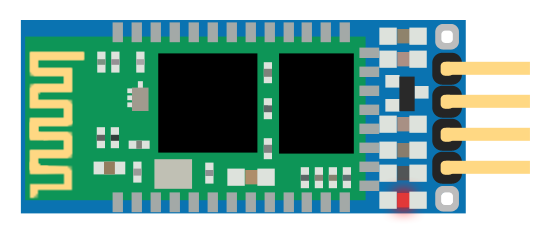
\includegraphics[width=0.8\textwidth]{modulo.png}
	\caption{Exemplo do módulo \textit{Bluetooth} utilizado pelo grupo de pesquisadores do Instituto Federal de Educação, Ciência e Tecnologia de Minas Gerais (IFMG - Campus Formiga).}
	\label{fig:modulo}
\end{figure}

Também, em sua extremidade esquerda , na ondulação vertical, é possível ver o emissor/receptor de ondas de rádio.

\subsection{Conceitos básicos sobre a tecnologia}
Primeiramente, deve-se verificar se os dispositivos possuem o \textit{software} do \textit{hardware} esteja atualizado. É um pré-requisito que muitos usuários não estão cientes que poderá acumular problema na sincronozação (\textit{pareamento}). Ambos os dispositivos deves estar habilitado ao \textit{pareamento}. Em telefones móveis, método semelhante a maioria dos dispositivos, basta definir a configuração para `habilitado' ou 'ligado' ou algo do gênero.

Nem todos os dispositivos podem ser \textit{empareados} qualquer outro dispositivos que também tenha \textit{Bluetooth}. Você não obterá sucesso ao \textit{parear} uma impressora a um fone de ouvido. Eles \textit{não foram projetados} pelos seus fabricantes para que isso possa ocorrer.


\subsection{Exemplo simples de sua aplicação em um programa}
Um exemplo para a aplicação de um programa básico deve-se, primeiramente, transferir todo o programa desejado para o Arduino indicando qual porta \textit{serial} (RX e TX) será utilizada. Nesta transferência, o módulo \textit{Bluetooth} não poderá estar conectado, pois ele, enviará o código ao \textit{Bluetooth} que não estará configurado ainda para sua função ainda.

Após o envio do código, deve-se desligar o Arduino e conectar os fios necessários entre o módulo \textit{Bluetooth} e o Arduino na seguinte sequência:

\begin{description}
\item[Pino VCC:] Na alimentação 3.6V até 6V
\item[Pino GND:] GND
\item[Pino TXD:] Digital 0
\item[Pino RXD:] Digital 1
\end{description}

Após este feito, é necessário que \textit{empareie} os dispositivos usando a senha para conexão \textbf{1234}. Esta senha é padrão para que possa enviar dados entre si. Normalmente, o nome padrão do dispositivo para \textit{empareamento} é \textbf{linvor} então é necessário que algum dos dispositivos disponíveis para uma primeira conexão para testes ou para configuração tenha este nome.

Após feito todos estes processos o programa estará pronto para executar a sua função sem a necessidade de fio para a conexão via \textit{serial}. 


\begin{figure}[h]
	\includegraphics[width=1.1\textwidth]{arduino.png}
	\caption{Exemplo de um Arduino Uno conetado a um Módulo \textit{Bluetooth}.}
	\label{fig:arduino}
\end{figure}

\subsection{Implementação no projeto do Carro Robô}

O dispositivo \textit{Bluetooth} foi utilizado no Projeto de Iniciação Científica do grupo para aumentar a dinâmica do espaço percorrido do Carro Robô. Utilizando a rede local produzida pela conexão para a transmissão de dados, ele não precisará de cabos que liguem a qualquer base (a energia necessária será carregada pelo próprio chassi do carro) permitindo o carro se locomova entre obstáculos como pequenas aberturas ou grandes distâncias (dentro do limite pré-estabelecidos) sem qualquer problema.

Além de baterias no seu interior, o carro também conterá o dispositivo receptor/rementente de radiofrequência e sensores que serão adicionados futuramente se o grupo estiver com o tempo adiantado (ao final das etapas do projeto). Além de comandos direcional como direita/esquerda e frente/retroceder, o carro deverá enviar dados de sua situação em que ele se encontra para o seu piloto (usuário) para que ele decida o que fazer. Ou até mesmo para que ele faça alguma ação de segurança evitando seu estrago ou algo do gênero quando o piloto não perceber a gravidade.

Após a conexão do módulo \textit{Bluetooth} com o Arduino (não sendo necessiariamente o Uno. Qualquer um que seja derivado destes microcontrolador poderá obterá sucesso) é identica ao da figura mencionada acima (Figura \ref{fig:arduino}).

Utilizando o \textit{software} desenvolvido, ele enviará os dados via serial pelos pinos RX, TX do Arduino e o módulo \textit{Bluetooth} encarregará de enviar para o dispositível móvel conectado e vice-versa.




%%%%%%%%%%%%%%%%%%%%%%%%%%%%%%%%%%%%%%%%%%%%%%%%%%%%%%%%%%%%%%%%%%%%%%%%%%%%%%%%%%%%%%%%%%%%%%%%
%                                                                                              %
%                               Nova Seção do Documento                                        %
%                                                                                              %
%%%%%%%%%%%%%%%%%%%%%%%%%%%%%%%%%%%%%%%%%%%%%%%%%%%%%%%%%%%%%%%%%%%%%%%%%%%%%%%%%%%%%%%%%%%%%%%%

\newpage
%%%%%%%%%%% Example %%%%%%%%%%%%%%%%%%%%%%%%%%
\section{Bibliografia}
\begin{thebibliography}{100} % 100 is a random guess of the total number of 

%references
\bibitem{robo} roboToSH. Acessado 22/10/2013. Disponível em: http://robotosh.blogspot.jp/2012/07/arduino-jy-mcu-\textit{Bluetooth}.html.

\bibitem{wiki} Arduino - \textit{Bluetooth} HC-05. Acessado 19/10/2013. Disponível em: http://www.tuxti.com.br/wiki/index.php/Arduino\_-\_Bluetooth\_HC-05

\bibitem{seguranca} See why \textit{Bluetooth} technology is simple, secure, everywhere. Acessado 19/10/2013. Disponível em: http://www.bluetooth.com/Pages/Simple-Secure-Everywhere.aspx
\end{thebibliography}

\end{document}